\section{Sprint 1}
Im ersten Sprint wurde der Grundstein für das Projekt sowie die Applikation gelegt.
Dies beinhaltete folgende Stories:
\begin{itemize}
   \item Teile des \ac{ATS} Codes sollen übernommen werden, so dass die Kommunikation mit Stromzählern möglich ist.
% in ADO gibt es no eine zweite story zur kommunikation, diese wird hier weggelassen
   \item Die Applikation DlmsQuickAccess soll so an Benutzer ausgeliefert werden, dass diese automatisch neue Updates erhalten.
   \item Die Applikation soll auf \ac{ADO} bei jedem neuem Commit automatisch gebaut und getestet werden. 
   \item Es soll eine Benutzerschnittstelle erstellt werden, welche alle Objekte eines Zählers auflistet.
% in ADO gibt es eine extra story zum ObjectModel parsen, diese wird hier weggelassen
\end{itemize}
In den folgenden Abschnitten werden die genannten Stories einzeln ausführlich beschrieben.
Als erstes wird jeweils das Ziel der Story genauer festgehalten.
Darauf folgend wird beschrieben wie die Story bearbeitet wurde, welche Schwierigkeiten aufgetreten sind und in welchem Zustand sich die Story zum Ende des Sprints befand.

\subsection{Implementation der Kommunikation mittels ATS Code}\label{s1:ats}
\dq Teile des \ac{ATS} Codes sollen übernommen werden, so dass die Kommunikation mit Stromzählern möglich ist.\dq

\subsubsection{Ziel}
Nebst des Codes für die Kommunikation mit Stromzähler beinhaltet das Projekt des \ac{ATS} viele weitere Komponenten wie beispielsweise eine Benutzerschnittstelle für das Verwalten von Testscripts oder einen Interpreter für die eigene Scriptsprache.
Die Story gilt als erledigt, wenn eine erfolgreiche Kommunikation mit einem Stromzähler durchgeführt werden kann.
Dabei soll nur jener Code, welche effektiv für die Kommunikation zuständig ist, in die DlmsQuickAccess Solution eingebunden werden. 


\subsubsection{Vorgehen und Schwierigkeiten}\label{atsUmsetztung}
Als erstes wurde der ATS Code analysiert.
Dabei zeigte sich, dass alle Klassen des \ac{ATS} in einem einzelnen C\# Projekt mit dem Namen \textit{Befehlsinterpreter} abgelegt sind.
Nebst den benötigten \ac{DLMS} Kommunikationskomponenten beinhaltet dieses Projekt auch Code für Benutzerschnittstellen sowie diversen andere Kommunikationsprotokolle.
Eine saubere Trennung der einzelnen Komponenten ist nicht erkennbar. 
Dies bestätigen auch die Code Metrics Results\footnote{https://docs.microsoft.com/en-us/visualstudio/code-quality/code-metrics-values?view=vs-2022}, sichtbar in Abbildung \ref{fig:codemetrics}.
\begin{figure}[H]
   \centering
   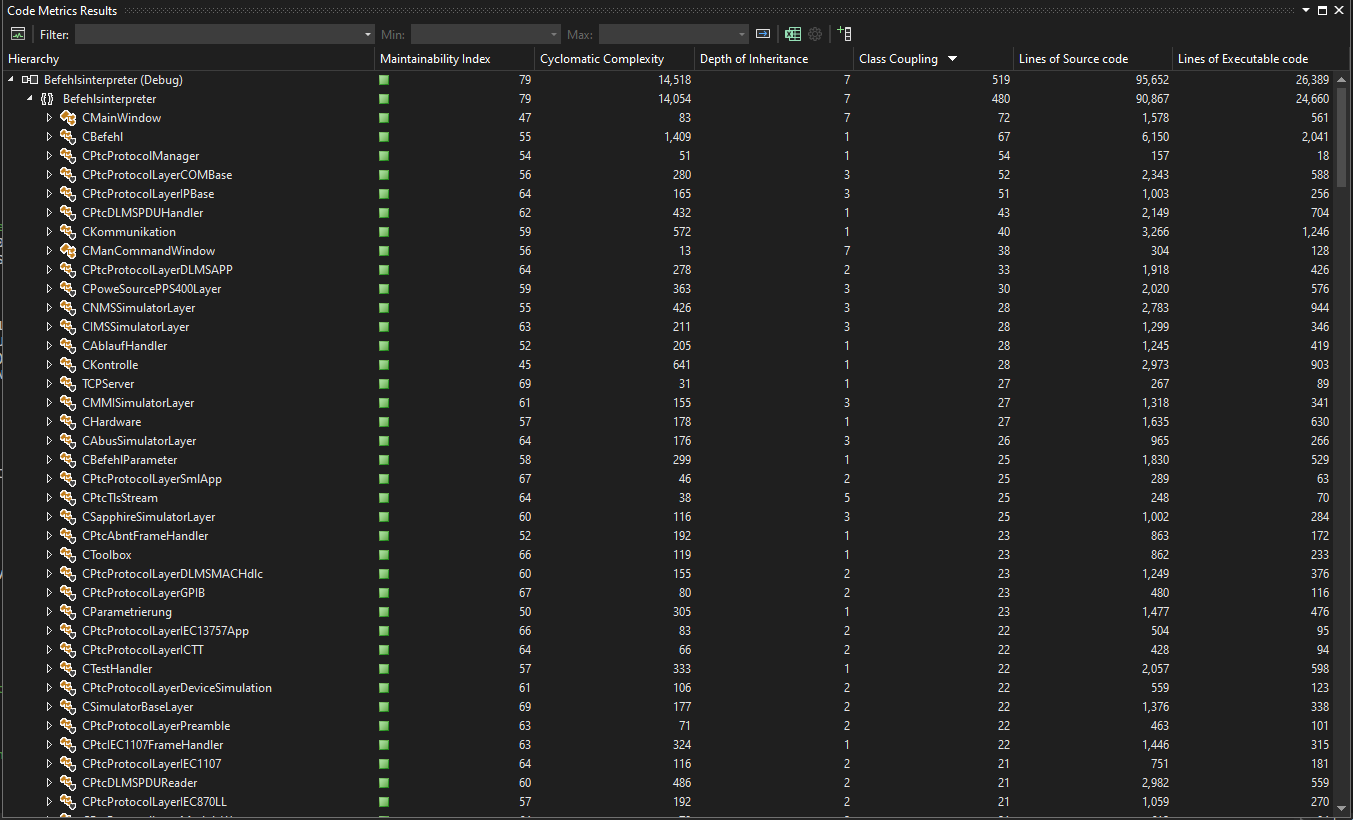
\includegraphics[width=1.0\textwidth]{gfx/S1_CodeMetrics_Befehlsinterpreter.png}
   \caption{
      Code Metrics zum Befehlsinterpreter Projekt
      }
      \label{fig:codemetrics}
\end{figure}
Einzelne Klassen sind mit bis zu 71 anderen gekoppelt, während laut \citeauthor{quantitativeInvestigationRiskCodeMetrics} (\citeyear{quantitativeInvestigationRiskCodeMetrics}) neun eine gute Obergrenze wäre.
Abbildung \ref{fig:codemetrics} zeigt des Weiteren, sowohl englische wie auch deutsche Klassennamen verwendet werden.
Aufgrund des Projektaufbaus ist es nicht möglich, den \ac{ATS} Code als Bibliothek mittels eines NuGet\footnote{https://docs.microsoft.com/en-us/nuget/what-is-nuget} Paketes einzubinden.
Im Kapitel \ref{ausblick:ats_split} wird jedoch darauf hingewiesen, dass es in der Zukunft sinnvoll sein könnte,
das Befehlsinterpreter Projekt aufzuspalten und einzelne Komponenten als Bibliotheken bereitzustellen.

Das Aufräumen der \ac{ATS} Projekts nicht teil dieser Arbeit sein soll, wurde versucht, nur jene Teile des Codes einzubinden, welche tatsächlich gebraucht werden.
So wurde das Repository des \ac{ATS} mittels Git Subtree\footnote{https://www.atlassian.com/git/tutorials/git-subtree} in das DlmsQuickAccess Repository eingebunden. 
Dies ermöglichte es, dass Klassen und Funktionen, welche nicht benötigt werden, entfernt werden konnten.
Die Änderungen am \ac{ATS} Code mussten lediglich in das Repository dieser Arbeit gepusht werden.
Wäre anstelle von Git Subtree Git Submodule verwendet worden, wäre dies nicht möglich gewesen.
Neue Versionen des \ac{ATS} Code können ebenfalls gepullt und gemerget werden. 
Der Nachteil dieses Ansatzes ist es, dass es etwas schwieriger ist, die gemachten Änderungen zum Ursprungsrepository zu pushen \parencite{gitSubtree}.
Da die geplanten Änderungen jedoch nur das Löschen von Code beinhalten, ist dieser Nachteil nicht relevant.

Die Klasse \textit{ReaderWriter} wurde geschrieben, um den Zugriff auf den \ac{ATS} Code an einem Ort zu bündeln.
Diese kümmert sich um das laden benötigter Konfigurationen, initialisiert die \ac{DLMS} Kommunikation und bietet eine Methoden zum Lesen und Schreiben von Daten an, welche von der Applikation benutzt werden kann.
\begin{figure}[H]
   \centering
   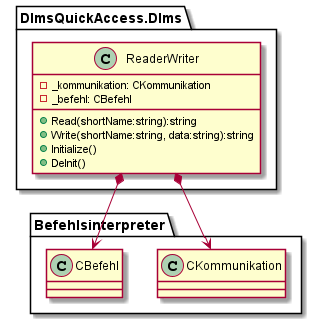
\includegraphics[width=0.5\textwidth]{gfx/readerwriter.png}
   \caption{
      Unvollständiges Klassendiagramm zur ReaderWriter Klasse
      }
      \label{fig:readerwriter}
\end{figure}
Sie ist im Klassendiagramm \ref{fig:readerwriter} abgebildet.
Die Kompositionen zu \textit{CBefehl} und \textit{CKommunikation} zeigen die Abhängigkeit zum \ac{ATS} Code.


% TODO schreiben wie der Stand ende S1 aussah

\subsection{Deployment}
\dq Die Applikation DlmsQuickAccess soll so an Benutzer ausgeliefert werden, dass diese automatisch neue Updates erhalten.\dq

\subsubsection{Ziel}
Obwohl die Anwendung zu diesem Zeitpunkt noch über keinerlei Funktionen verfügt, welche für einen Benutzer nützlich sein könnten, soll das Deployment der Applikation bearbeitete werden.
Damit wird sichergestellt, dass WinUI3 Applikationen in der Umgebung der Landis+Gyr korrekt ausgeliefert werden können.
Dies ist wichtig, da es in der Vergangenheit bei der Auslieferung von Anwendungen Probleme mit restriktiven Sicherheitsrichtlinien gab.

Die Story gilt als abgeschlossen wenn es für einen Benutzer möglich ist die Applikation eigenständig zu installieren.
Updates, welche nach dem Installationszeitpunkt erscheinen, sollen automatisch aufgespielt werden.

\subsubsection{Vorgehen und Schwierigkeiten}
Da die Anwendung nur intern bei der Landis+Gyr verwendet werden wird und somit nicht über eine offizielle Quelle verteilt werden, muss sie via Sideloading installiert werden \parencite{sideload}.
Die Entwicklungsumgebung Visual Studio 2022 Enterprise, welche für die Entwicklung der Anwendung verwendet wurde, ermöglicht es Packages fürs Sideloading zu erstellen.
Über einen Dialog werden dabei Konfigurationen wie Versionsnummer, Ausgabepfad oder Prozessorarchitektur angegeben.
Die Anwendung soll auf einem Netzwerkverzeichnis abgelegt werden, auf welches alle Entwickler Zugriff haben.
Dieses wir auch für die Verteilung andere Programme wie beispielsweise der Compiler der Firmware verwendet.

Eine erste, leere Version des DlmsQuickAccess konnte einfach gebaut und über die beschriebene Funktion von Visual Studio auf das Netzwerkverzeichnis deployt werden.
Die dabei erstellte Datei \textit{DlmsQuickAccess (Package).appinstaller} konnte auf dem Rechner des Entwicklers problemlos ausgeführt und die Anwendung somit installiert werden.
Nach der ersten erfolgreichen Installation wurde eine zweite Version veröffentlicht, um zu testen, dass sich die Anwendung automatisch aktualisiert.
Dies funktioniert so, dass der DlmsQuickAccess beim jedem Start überprüft, ob sich auf dem Netzwerkverzeichnis eine neue Version befindet.
Falls dies so ist wird diese heruntergeladen und beim nächsten Schliessen der Anwendung installiert.

Erste Probleme traten auf, als versucht wurde, die Installation auf einem Rechner eines anderen Benutzers durchzuführen.
Die Signatur der Anwendung konnte nicht überprüft werden, da diese mit einem Schlüssel erstellt wurde, welcher lokal auf dem Rechner des Entwicklers erstellt wurde.
Damit die Signatur erfolgreich validiert werden kann, muss der öffentliche Schlüssel beim Zielcomputer als \textit{Trusted Root Certificate Authorities} hinterlegt werden.
Eine Alternative wäre anstelle des selbst signierten Zertifikat eines zu verwenden, das von einer Certification Authority ausgestellt wurde.
Ein solches konnte die Landis+Gyr für dieses Projekt jedoch nicht zeitnah zur Verfügung stellen.
Im Kapitel \ref{ausblick:cert} wird dies als offener Punkt festgehalten.

\begin{figure}
   \centering
   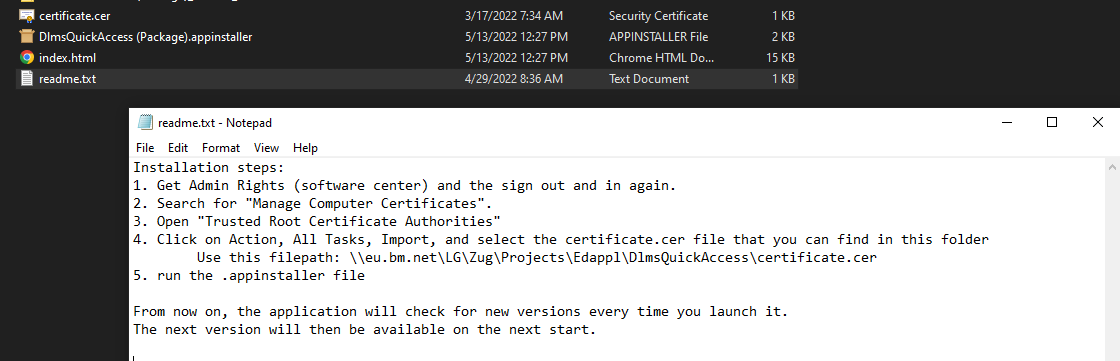
\includegraphics[width=1.0\textwidth]{gfx/installer_readme.png}
   \caption{
      Netzwerkverzeichnis mit Installer, Zertifikat und geöffneter Installationsanleitung
      }
      \label{fig:installerreadme}
\end{figure}

Um den Installationsprozess für die Benutzer möglichst einfach zu gestalten, wurde der öffentliche Schlüssel sowie eine Schritt-für-Schritt Anleitung auf dem Netzwerkverzeichnis abgelegt.
Diese sind in Abbildung \ref{fig:installerreadme} zu sehen.


\subsection{Build bei Commit}\label{story_buildoncommit}
\dq Die Applikation soll auf \ac{ADO} bei jedem neuem Commit automatisch gebaut und getestet werden.\dq

\subsubsection{Ziel}
Die \ac{CI} Umgebung auf \ac{ADO} soll so konfiguriert werden, dass bei jeder neuen Änderung geprüft wird, ob diese valid ist und keine bestehenden Funktionen bricht.
Die Story gilt als erledigt, wenn bei jedem Commit automatisch ein vollständiger Build erstellt wird und alle UnitTests ausgeführt werden.

\subsubsection{Vorgehen und Schwierigkeiten}
Bei dieser Story traten diverse Schwierigkeiten auf.
Einige hatten damit zu tun, wie die \ac{ADO} Instanz der Landis+Gyr verwaltet wird.
Um beispielsweise ein neues Projekt zu erstellen oder zusätzliche Berechtigungen zu erhalten musste jeweils ein Ticket erstellt werden, welches zuerst von einem Manager genehmigt werden musste und danach vom Verwalter der \ac{ADO} Instanz bearbeitet wurde.

Zuerst musste ein solches Ticket erstellt werden, um Zugriff auf die Build Pipeline zu erhalten.
In einem zweiten erhielt die Pipeline Zugriff auf einen Windows Build Agent.
Ein drittes Ticket war nötig, um auf dem Agent die neuste Version von Visual Studio Enterprise zu installieren.

Da die Person, welche die Tickets bearbeitet während dieses Sprint noch eine Woche in den Ferien war, war die benötigte Visual Studio Version erst zu Beginn des zweiten Sprints verfügbar.
Diese Story konnte somit nicht geschlossen werden.
Wie sie im zweiten Sprint weitergeführt wurde, ist in Abschnitt \ref{s2:buildOnCommit} zu lesen.


\subsection{Darstellung des Object Model}\label{visualizeOM}
\dq Es soll eine Benutzerschnittstelle erstellt werden, welche alle Objekte eines Zählers auflistet.\dq

\subsubsection{Ziel}
Eine zentrale Funktion des zu ersetzenden \textit{Quick Access} ist die visuelle Auflistung aller Objekte eines Stromzählers.
In der neuen Applikation wird eine solche ebenfalls benötigt.
Die Story gilt als erledigt, wenn folgende Elemente der Objekte vollständig angezeigt werden:
\begin{itemize}
   \item Der Name des Objekts
   \item Die ClassId inklusive Version, Own Class Version und Sub Type
   \item Der Name und die Id aller Attribute und Methoden
\end{itemize}

\subsubsection{Vorgehen und Schwierigkeiten}\label{objectModelDevSchwierigkeiten}
Die Object Models, welches in dieser Story dargestellt werden sollen, sind als XML Dateien verfügbar (mehr dazu im Abschnitt \ref{objectModelsClassDescriptions}).
Um die Daten in der Benutzerschnittstelle darzustellen, müssen diese zuerst in einer Klassenstruktur vorhanden sein.
Der Code der in Abschnitt \ref{objectModelsClassDescriptions} beschriebenen Software \textit{PicassoTools} bietet eine solche an.
Diese ist für diese Anwendungen jedoch ungeeignet, da sie nicht das logische Object Model repräsentiert, sondern die Tabellenform dessen.
So enthält sie beispielsweise angaben zu Reihen und Spalten der einzelnen Objekte.
Deshalb wurde eine neue Struktur entworfen, welche auf die Anforderungen des DlmsQuickAccess zugeschnitten ist.
Das Diagramm in Abbildung \ref{fig:objectModelInterface} zeigt deren Interfaces.

\begin{figure}
   \centering
   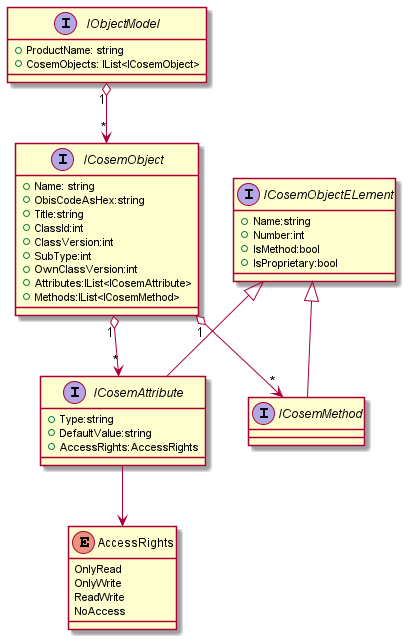
\includegraphics[width=0.7\textwidth]{gfx/ObjectModel_interfaces.png}
   \caption{
      Klassendiagramm zu den Interfaces des Object Models
      }
      \label{fig:objectModelInterface}
\end{figure}

Um die XML Dateien in der Applikation zu verarbeiten wurde ein Parser geschrieben, welcher die XML Datei liest und in die gezeigte Klassenstruktur abbildet.
Da der Parser die erste Klasse war, welche für dieses Projekt implementiert wurde, wurde auch erste Unit Tests benötigt.
Dazu musste ein passendes Testing- sowie Mocking-Framework gewählt werden.
Bei ersterem viel die Wahl auf MSTest \footnote{https://docs.microsoft.com/en-us/dotnet/core/testing/unit-testing-with-mstest}, da dieses bereits in mehreren anderen C\# Projekten der Landis+Gyr verwendet wird.
Für die Wahl des Mocking-Framework wurde die Syntax mehrerer Optionen verglichen \parencite{clarke_2020}.
Dabei konnte jene von Moq \footnote{https://github.com/moq/moq4} am meisten überzeugen.

Im Abschnitt \ref{aufbauUI} wurde der grundlegende Aufbau der Benutzerschnittstelle erklärt.
Die Darstellung des Object Models, ist der erste Teil dieses Konzepts, der in die Anwendungen umgesetzt wird.
Um bei der Realisierung der Benutzerschnittstelle strukturiert vorgehen zu können, wurden Rastersysteme eingesetzt.
Diese erweitern den Sktech, welcher in Abbildung \ref{fig:objectModelUIsktech} gezeigt ist, um konkrete Angaben zu den Spaltenbreiten.
In den Abbildungen \ref{fig:singleObjectTitleGrid} und \ref{fig:singleObjectContentGrid} sind einige Beispiel aufgeführt.

\begin{figure}
   \centering
   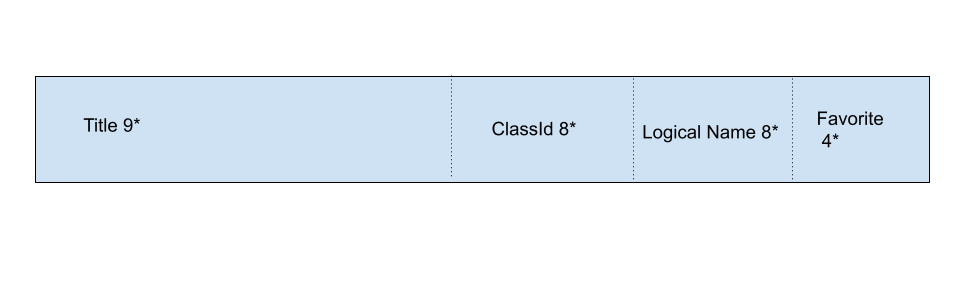
\includegraphics[width=1.0\textwidth]{gfx/Single Object Title Line Grid.png}
   \caption{
      Rastersystem zum Titel eines einzelnen Objekts
      }
      \label{fig:singleObjectTitleGrid}
\end{figure}

\begin{figure}
   \centering
   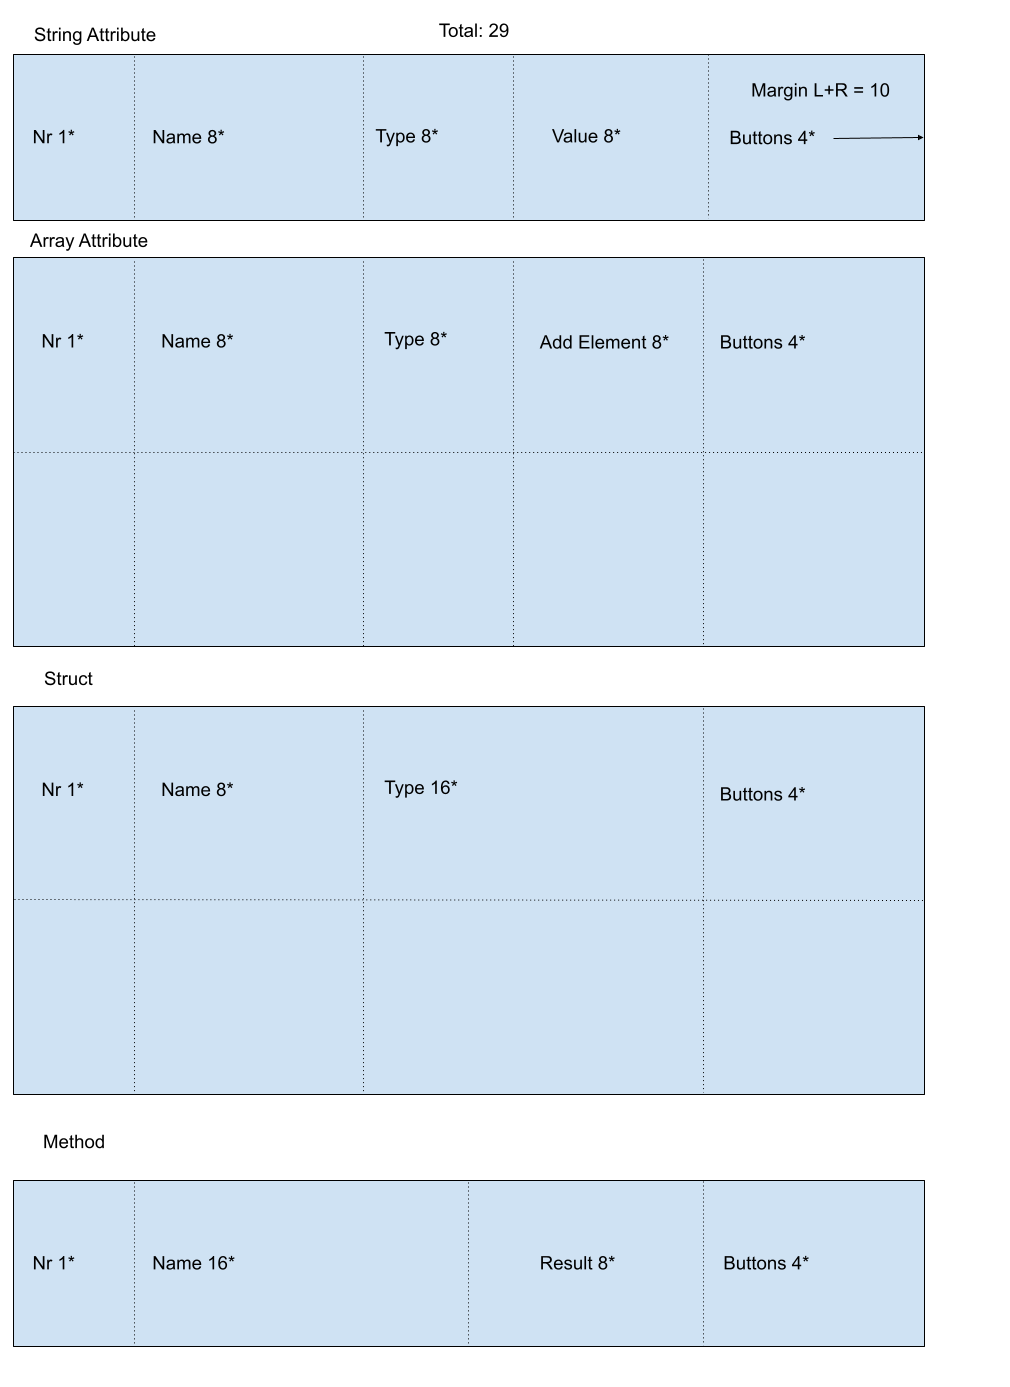
\includegraphics[width=1.0\textwidth]{gfx/Single Object Content Grid.png}
   \caption{
      Rastersysteme zum unterschiedlichen Arten von Attributen/Methoden
      }
      \label{fig:singleObjectContentGrid}
\end{figure}


Für die Implementation der Benutzerschnittstelle wird, wie in \ref{mvvm} beschrieben, das Muster \ac{MVVM} verwendet.
Das Model besteht in diesem Fall aus der zuvor erwähnten Klassenstruktur, welche das Object Model repräsentiert.
Für die View wurde die Klasse \textit{ObjectModelControl} erstellt, in welcher die eigentliche Benutzeroberfläche mittels XAML deklariert wird.
Um die Objekte, Attribute und Methoden hirarchisch darzustellen, wurden  \textit{TreeView} \footnote{https://docs.microsoft.com/en-us/windows/winui/api/microsoft.ui.xaml.controls.treeview?view=winui-3.0} Controls der WinUI3 Library verwendet.
Die Klasse \textit{ObjectModelViewModel}, welche das \ac{MVVM} Muster komplettiert, beinhaltet Properties, welche in der View mittels DataBinding angezeigt werden.

Während diesen Arbeiten trat folgendes Problem auf.
Um eine WinUI3 Applikation zu bauen muss eine Windows Version angegeben werden, welche minimal unterstützt werden soll.
Dies wird mit dem Property \textit{TargetFramework} im Projektfile gemacht.
Bei klassischen C\# Projekten wird dort lediglich die Version des .net Frameworks, beispielsweise \textit{net6.0} spezifiziert.
Für WinUI3 muss diese noch um die Windows Version ergänzt werden. Dies sieht dann so aus: \textit{net6.0-windows10.0.19041.0}.
Damit ein Test Projekt eine Dependency auf ein reguläres Projekt mit der eben genanntem \textit{TargetFramework} haben konnte, musste dieses das selbe \textit{TargetFramework} spezifizieren, sonst gab es einen Kompilerfehler.
Der Kompilerfehler verschwindet, wenn das \textit{TargetFramework} angepasst wird. Dies führt jedoch dazu, dass die Tests nicht mehr ausgeführt werden.
Diese Problem konnte so gelöst werden, dass die zu testenden Klassen nicht in jenem Projekt abgelegt wurden, welches die Referenz zu WinUI3 hat.
Der Nachteil dabei ist, dass Code, welcher eine Abhängigkeit zu WinUI3 hat nicht automatisiert getestet werden kann.
Dies kann jedoch akzeptiert werden, da es dabei nur um Control Klassen handeln wird, welche lediglich deklarativen XAML Code enthalten.
\subsection{Logging}
Um in einem Fehlerfall nachvollziehen zu können wann und wieso das Progamm abgestützt ist, wurden Logging Nachrichten in verschiedene Teile der Software eingebaut.
Dazu wurde das Logging Framework \textit{log4net} verwendet, da dieses auch in anderen C\# Projekten der Landis+Gyr eingesetzt wird.
Dieses konnte mit Hilfen von StackOverflow\footnote{https://stackoverflow.com/questions/53092470/how-to-configure-logging-via-log4net-in-an-uwp-app} für die Applikation konfiguriert werden.

\subsection{Globaler Exception Handler}

Exceptions, welche vom Programm nicht abgefangen werden und zu einem Absturz der Anwendung führen, werden von einem globalen Exception Handler gefangen.
Dieser schreibt deren auftreten in die Log-Datei. Für vereinfachtes Troubleshooting, wir diese Log Datei auch sofort geöffnet. Das Programm stürzt danach ab.
Es musste festgestellt werden, dass nicht ganz alle Ausnahmen so behandelt weren können\footnote{https://docs.microsoft.com/en-us/windows/winui/api/microsoft.ui.xaml.application.unhandledexception?view=winui-3.0}.
Exceptions, welche im Aufbau der Anwendung vorkommen, also beispielsweise im XAML oder im Konstruktor eines ViewModels können nicht abgefangen werden.


\pagebreak

